
\documentclass[brazilian,12pt,a4paper,final]{article}


\usepackage[a4paper,
bindingoffset=0.2in,
left=0.8in,
right=0.8in,
top=0.8in,
bottom=0.8in,
footskip=.25in]{geometry}

%% Pacotes extras (opcionais):

% *babel* contem as regras de hifenização
\usepackage[portuguese]{babel}
% *t1enc* permite o reconhecimento dos acentos inseridos com o teclado
\usepackage{t1enc}

% *inputenc* com opção *utf8* permite reconhecimento dos caracteres com codificação UTF8, que é padrão dos esditores de texto no Linux. Isso permite reconhecimento automático de acentuação.
%\usepackage[utf8]{inputenc}
\usepackage{epsfig}

% *graphicx* é para incluir figuras em formato eps 
\usepackage{graphicx} % para produzir PDF diretamente reescrever esta linha assim: \usepackage[pdftex]{graphicx}

% *color* fontes soloridas
\usepackage{color}
%%% fim do cabecalho %%%

\pagestyle{empty}
\title{Métodos Computacionais Aplicados à Biocomplexidade}
\author{Aluno: André Gustavo Dessoy Hubner - Matrícula: 00315569 \\ IF-UFRGS}

\begin{document}
	\maketitle
	
	\section{Introdu\c{c}\~ao} 
	% Aqui a Introdução \c{c} e \~a  é a forma standar  de escrever
	% carateres ASCII extendidos (acentos, etc), porem com o pacote t1enc
	% declarado acima podemos escrever diretamente ç em lugar d \c{c}, etc
	\indent 
	Este documento relata a criação de uma rede metabólica entre compostos de reações de enzimas registradas ao \textit{Echinops telfairi} nas bases de dados KEGG, assim como a comparação de algumas de suas propriedades com um grafo aleatório, buscando no processo entender as idiossincricidades de um grafo desse tipo.
	
	\section{Metodologia}
	\subsection{Busca de enzimas, suas reações e cada composto}
	A KEGG conta com uma API disponibilizando diversos métodos para obter os dados que ela contém através de um programa. O primeiro passo nesse projeto foi a escolha de um organismo com o qual trabalhar, o que foi feito primeiramente com a operação "list" da API tendo como alvo a base de dados "organism", listando organismos disponíveis no KEGG como um todo e que contêm códigos de três a quatro letras. Para realizar essa e todas as outras requisições subsequentes, utilizei o método "urlopen", pertencente ao módulo "request" da biblioteca "urllib". A partir do retorno em string dessa listagem, testei os retornos de enzimas e reações subsequentes de algumas deles e após indas e vindas decidi trabalhar com 	
	\textit{Echinops telfairi}, um ouriço endêmico ao Madagascar, de côdigo etf.
	\vspace{0.5cm}
	
	A próxima operação realizada foi "find", tendo como alvo a base "enzyme" e o código etf para buscar por enzimas registradas especificamente para \textit{Echinops telfairi}. Com essa requisição, foi possível então obter 6 enzimas cujos códigos seriam usados para buscar por suas reações, desta vez utilizando a operação "link" seguida por um parâmetro para buscar na base "reaction" e, por fim, o código da respectiva enzima como valor de query (consulta). 
	\vspace{0.5cm}
	
	O que a operação "link" faz de especial é buscar os resultados através de referência cruzada, ou seja, ao invés de usar "find" para buscar diretamente na base "reaction" por reações, o que se faz é buscar por cada uma delas através das referências das enzimas em si, sendo portanto uma operação mais próxima do nosso objetivo de buscar resultados provenientes das enzimas. Assim, a busca foi feita para cada enzima e os resultados processados para filtrar pelos códigos desejados, por fim armazenando-os assim como as enzimas. Ao final, foram obtidas 6 reações.
	\vspace{0.5cm}
	
	A última operação de busca realizada também foi a de "link", porém agora tendo a base "compound" como alvo e usando como valor de query cada uma das reações encontradas no passo acima. Assim como no caso anterior, também foi necessário filtrar as strings dos resultados pelo código relevante, através da biblioteca "re" para regex. Ao todo, foram obtidos 21 compostos das 6 reações, o que também significa que a nossa rede terá 21 nós. Na mesma função contendo toda a lógica para a busca e o armazenamento dos códigos dos compostos, também achei interessante escrever em um arquivo txt os compostos encontrados por reação, de forma a facilitar o observação dos resultados sem usar a ferramenta de debug.
	\vspace{0.5cm}
	
	As duas primeiras figuras demonstram como foram feitas as buscas e a obtenção dos códigos advindos dos resultados do KEGG, sendo a primeira sobre a busca das reações e a segunda sobre os compostos delas. Tendo todos os compostos, ainda era necessário construir a rede contendo a relação entre eles.
	
		
	\begin{figure}[hbtp]
		\begin{center}
			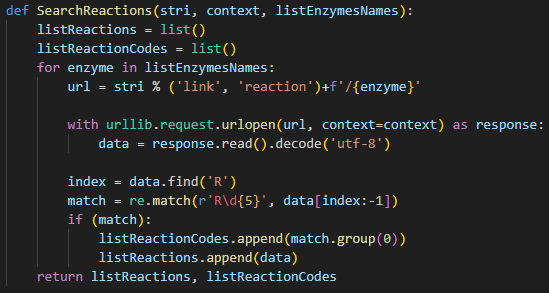
\includegraphics[]{SearchReactions.png}
			\caption{Função usada para buscar e extrair os códigos das reações desde as enzimas obtidas na etapa anterior.}
			\label{fig}
		\end{center}
	\end{figure}
	
		
	\begin{figure}[hbtp]
		\begin{center}
			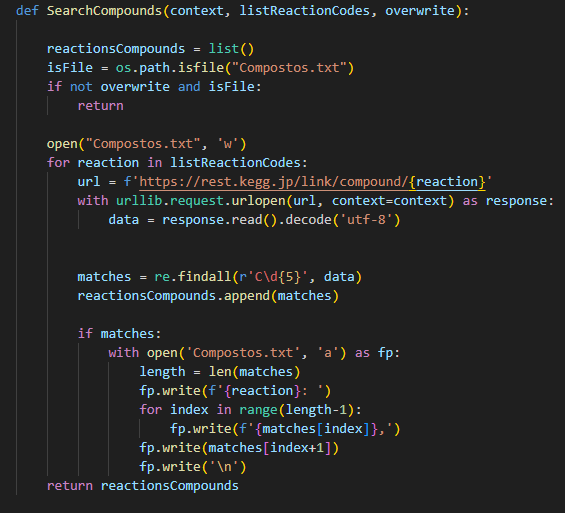
\includegraphics[]{SearchCompounds.png}
			\caption{Função usada para em cada reação obter todos os compostos e escrevê-los em um arquivo.}
			\label{fig}
		\end{center}
	\end{figure}
	
	\subsection{Obtenção dos graus de cada nó e construção da matriz}
	
	Tendo em vista que existem compostos repetidos para as reações, decidi armazenar os compostos em uma variável do tipo set, de forma a ter uma estrutura contendo todos os compostos sem redundância. Isso foi feito atualizando o conjunto do zero a partir de cada código de composto armazenado no arquivo criado pela função "SearchCompounds".
	\vspace{0.5cm}
	
	Outra estrutura importante que ainda era necessária é um dicionário contendo as reações de que cada composto participa. para construí-lo, uma vez que o retorno de SearchCompounds continha listas de todos os compostos para cada reação, bastou iterar pela variável representando-o e por cada composto dentro de cada lista, criando o índice no dicionário caso ainda não existisse para aquele composto e adicionando a respectiva reação. Este dicionário foi armazenado na variável "compoundsReactionsDict".
	\vspace{0.5cm}
	
	Finalmente, para a construção da matriz de adjacência representando uma rede com arestas entre nós relacionados por reações, foi utilizada uma lógica básica de matriz. A matriz terá um número igual de linhas e colunas, uma vez que cada um é representado pelo número de nós. Se itera por cada coluna em cada linha, verificando primeiro se o composto da linha e da coluna não é o mesmo, inserindo um grau de 0 nessa posição. Caso contrário, o grau dessa posição será calculado pela função "GetDegree", que recebendo os compostos representados pela atual linha e coluna e a referência ao dicionário "compoundsReactionsDict", essencialmente iterará pelos valores dos índices dizendo respeito à linha e coluna atual, adicionando 1 ao grau para cada valor entre eles que esteja contido em ambas as listas de reações. A próxima figura mostra o excerto do código contendo essa parte.
	
	\begin{figure}[hbtp]
		\begin{center}
			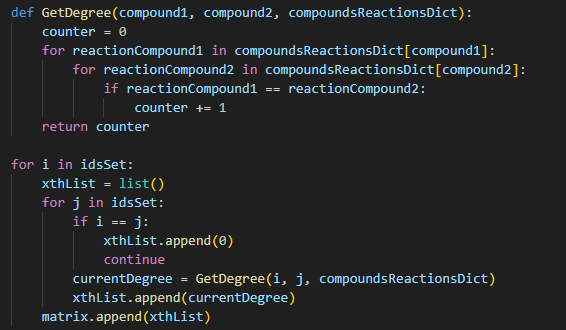
\includegraphics[]{Matriz.png}
			\caption{Passo do código contendo a construção da matriz de adjacência e a obtenção de cada grau que será inserido nela.}
			\label{fig}
		\end{center}
	\end{figure}
	
	\section{Resultados}
	
	As comparações realizadas aqui serão entre a rede construída anteriormente e uma rede aleatória, construída com a função "rand\_graph" conforme visto em aula.
	\vspace{0.5cm}
	
	Seguem duas tabelas com estatísticas relevantes para ambas as redes, assim como os grafos obtidos para os dois casos:
	\vspace{6cm}
	
	\begin{table}[]
		\begin{tabular}{|l|l|}
			\hline
			Coeficiente de clustering global & 0.642  \\ \hline
			Assortatividade                  & 0.0995 \\ \hline
			Total de links obtidos           & 71     \\ \hline
		\end{tabular}
		\caption{Estatísticas para a rede metabólica}
		
		\vspace{0.5cm}

		\begin{tabular}{|l|l|}
			\hline
			Coeficiente de clustering global & 0.586  \\ \hline
			Assortatividade                  & -0.731 \\ \hline
			Total de links obtidos           & 126     \\ \hline
		\end{tabular}
		\caption{Estatísticas para a rede aleatória}
	\end{table}
	
	
	\begin{figure}[hbtp]
		\begin{center}
			\includegraphics[width=10cm, height=10cm]{Grafo rede metabólica.png}
			\caption{Grafo obtido da matriz de adjacência construída através dos passos anteriores.}
			\label{fig}
		\end{center}
	\end{figure}
	
	\begin{figure}[hbtp]
		\begin{center}
			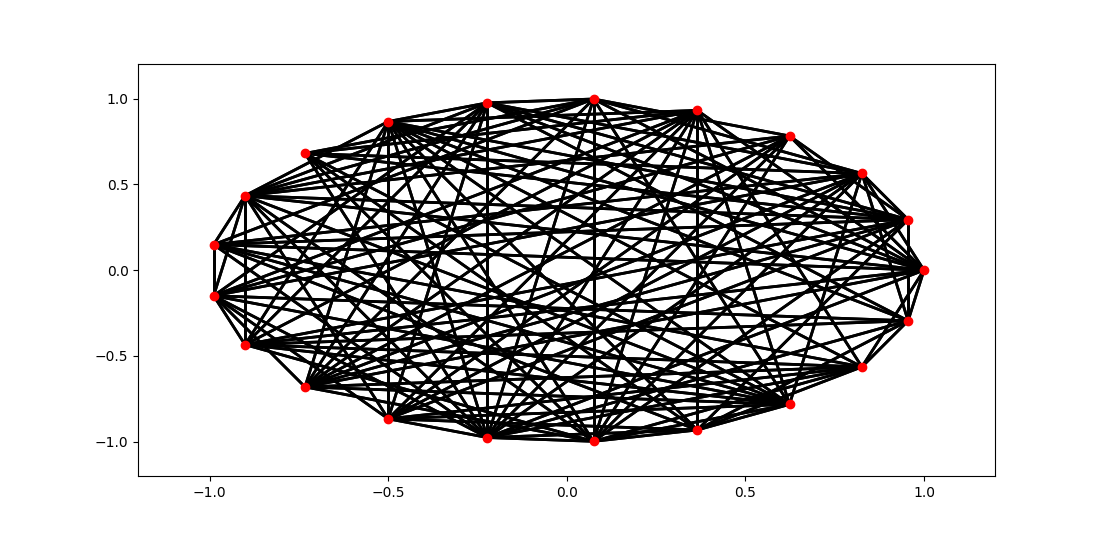
\includegraphics[width=10cm, height=10cm]{Grafo aleatório.png}
			\caption{Grafo obtido aleatoriamente.}
			\label{fig}
		\end{center}
	\end{figure}
	
	à primeira vista é notável que os links de rede metabólica estão alocados de maneira bem desproporcional pelo menos em relação à rede aleatória, sendo esta uma característica compatível com a matriz construída e os padrões em redes reais. É importante notar também que para os nós com maior número de links nessa rede o número real de links é ainda maior que o que é possível ver, uma vez que existem os mesmos compostos em mais de uma reação de \textit{Echinops telfairi}, o que na matriz é representado por números maiores que um. Devido a uma limitação da função de plot do gráfico, porém, esses links são desenhados um acima do outro, tornando as unidades a mais imperceptíveis.
	\vspace{0.5cm}
	
	Já sobre as estatísticas, os coeficientes de clustering globais das duas redes serem semelhantes é esperado, uma vez que o mesmo valor de clustering global obtido para a rede metabólica foi usada para gerar links na rede aleatória. Com esses valores, infere-se que em ambas as redes os nós tendem a ter metade dos possíveis links preenchidos nas suas regiões vizinhas.
	\vspace{0.5cm}
	
	Por outro lado, a assortatividade variou profundamente. Enquanto que para a rede metabólica há uma tendência bem pequena dos nós estarem ligados a outros nós com graus semelhantes, para a rede aleatória se verifica uma desassortatividade bem grande, com nós se relacionando com outros de graus diferentes. Embora possa-se pensar que essa diferença se dá por alguma propriedade específica de algum dos gráficos, na verdade parece estar associada à própria aleatoriedade do segundo caso, uma vez que executei o programa algumas vezes e em alguns casos foram gerados redes aleatórias com valores bem diferentes de assortatividade, inclusive semelhantes à rede metabólica.
	\vspace{0.5cm}
	
	Quanto à última estatística, o total de links obtidos na rede aleatória representou quase o dobro da rede metabólica, o que é um tanto surpreendente considerando os coeficientes de clustering semelhantes entre os dois. No momento de análise deste ponto, decidi alterar a função "clustering", usada para calcular o clustering de cada nó das duas redes, para tentar considerar o fato de dois nós poderem ter mais de um link, que é o caso da rede metabólica. Isso foi feito alterando a verificação de se há um link entre vizinhos de "M[jj][kk]==1" para "M[jj][kk]>=1". Com isso, em uma nova execução a primeira rede gerou um coeficiente de clustering de 0.821, um tanto mais alto que o original.
	\vspace{0.5cm}
	
	Por fim, os histogramas nas figuras 6 e 7 demonstram a distribuição dos graus dos nós de cada rede. Fica bastante claro, assim como esperado, que a rede metabólica, ao contrário da rede aleatória, apresenta uma distribuição bem mais desigual, com grande parte dos nós se relacionando com até 6 outros nós, enquanto não há nenhum no meio da distribuição e alguns com graus entre 15 e 19. A distribuição na rede aleatória é muito mais uniforme, o que é demonstrado pela distância entre o maior grau e o menor ser de apenas 8, e de praticamente toda posição entre eles haver pelo menos um nó com aquele grau.
	
	\begin{table}[]
		\begin{tabular}{|l|l|}
			\hline
			Coeficiente de clustering global & 0.821  \\ \hline
		\end{tabular}
		\caption{Coeficiente de clustering da rede metabólica atualizado após a atualização feita na funcão "clustering"}
	\end{table}
		
	\begin{figure}[hbtp]
		\begin{center}
			\includegraphics[width=10cm]{hist-rede-metabólica.png}
			\caption{Histograma representando a distribuição dos graus da rede metabólica.}
			\label{fig}
		\end{center}
	\end{figure}
	
	\begin{figure}[hbtp]
		\begin{center}
			\includegraphics[width=10cm]{hist-rede-aleatória.png}
			\caption{Histograma representando a distribuição dos graus da rede aleatória.}
			\label{fig}
		\end{center}
	\end{figure}
	
	\begin{figure}[hbtp]
		\begin{center}
			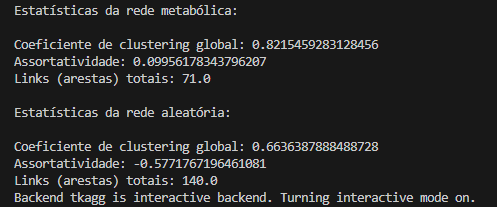
\includegraphics[width=10cm]{dadosAtualizados.png}
			\caption{Captura de tela demonstrando os resultados das estatísticas utilizando o print do Python após a modificação realizada na função "clustering". Há outros valores diferentes das tabelas 2, no entanto isso é devido a ser outra execução, sendo gerada portanto outra rede aleatória para a tabela 2.}
			\label{fig}
		\end{center}
	\end{figure}
	
	
	
	
	
	
	
	
	
	

	
	
\end{document}

